\documentclass[aspectratio=169,11pt]{beamer}

% Theme and Color Scheme
\usetheme{Madrid}
\usecolortheme{default}
\setbeamercolor{palette primary}{bg=blue!70!black,fg=white}
\setbeamercolor{palette secondary}{bg=blue!60!black,fg=white}
\setbeamercolor{palette tertiary}{bg=blue!80!black,fg=white}
\setbeamercolor{titlelike}{parent=palette primary}
\setbeamercolor{frametitle}{bg=blue!70!black,fg=white}
\setbeamertemplate{navigation symbols}{}
\setbeamertemplate{footline}[frame number]

% Packages
\usepackage[utf8]{inputenc}
\usepackage[T1]{fontenc}
\usepackage{amsmath}
\usepackage{amssymb}
\usepackage{graphicx}
\usepackage{booktabs}
\usepackage[table]{xcolor}
\usepackage{tikz}
\usepackage{hyperref}
\usepackage{subcaption}

\usetikzlibrary{positioning,shapes,arrows,calc}

% Custom colors
\definecolor{criticalred}{RGB}{220,50,50}
\definecolor{highyellow}{RGB}{255,180,50}
\definecolor{moderateblue}{RGB}{100,150,220}
\definecolor{lowgreen}{RGB}{80,180,100}

% Title Information
\title{ESG Stranded Assets Analysis}
\subtitle{Carbon Transition Risk in Copper Mining}
\author{Alexis Vannson, Kerrian Le Bars and Othmane Menkor}
\institute{Research Emerging Topics}
\date{January 2026}

\begin{document}

% SLIDE 1: Title
\begin{frame}
\titlepage
\begin{center}
\large{Quantifying Climate Transition Risk Across 914 Global Mining Assets}
\end{center}
\end{frame}

% SLIDE 2: Overview
\begin{frame}{Project Overview}
\begin{columns}[T]
\column{0.5\textwidth}
\textbf{Research Questions:}
\begin{itemize}
    \item Which copper mining assets become unprofitable under carbon pricing?
    \item What is the total financial exposure to carbon costs?
    \item How are emissions trending over time (2021-2024)?
    \item Can we predict stranded asset risk using machine learning?
\end{itemize}

\vspace{0.5cm}

\textbf{Scope:}
\begin{itemize}
    \item 914 mining assets globally
    \item 56+ countries analyzed
    \item 51,184 monthly emission records
    \item 4 carbon pricing scenarios (\$50-\$200/tCO\textsubscript{2})
\end{itemize}

\column{0.5\textwidth}
\textbf{Data Source:}
\begin{block}{Climate TRACE v5.2.0}
\begin{itemize}
    \item Satellite + AI emissions tracking
    \item Monthly data: Jan 2021 - Aug 2025
    \item Most comprehensive global emissions database
\end{itemize}
\end{block}

\vspace{0.5cm}

\textbf{Methodology:}
\begin{itemize}
    \item Financial risk modeling
    \item Machine learning predictions
    \item Interactive web dashboard
    \item Scenario stress testing
\end{itemize}
\end{columns}
\end{frame}

% SLIDE 3: The Problem
\begin{frame}{The Problem: Carbon Pricing Impact}
\begin{center}
\Huge \textcolor{criticalred}{\textbf{\$19.04 Billion}}

\vspace{0.5cm}

\Large Annual carbon cost exposure at \$200/tCO\textsubscript{2}

\vspace{1cm}

\normalsize
\begin{columns}[T]
\column{0.25\textwidth}
\centering
\textbf{914 Assets}\\
Global copper mines

\column{0.25\textwidth}
\centering
\textbf{56 Countries}\\
Worldwide coverage

\column{0.25\textwidth}
\centering
\textbf{259 Assets}\\
At critical/high risk

\column{0.25\textwidth}
\centering
\textbf{28.3\%}\\
Of assets vulnerable
\end{columns}

\vspace{1cm}

\textit{Carbon pricing will destroy value. The question is: how much?}
\end{center}
\end{frame}

% SLIDE 4: Key Findings - Financial Exposure
\begin{frame}{Key Finding \#1: Massive Financial Exposure}
\begin{columns}[T]
\column{0.5\textwidth}
\textbf{Carbon Cost by Scenario:}

\vspace{0.3cm}

\begin{table}
\small
\begin{tabular}{lr}
\toprule
\textbf{Scenario} & \textbf{Annual Cost} \\
\midrule
\$50/tCO\textsubscript{2} & \$4.76B \\
\$100/tCO\textsubscript{2} & \$9.52B \\
\$150/tCO\textsubscript{2} & \$14.28B \\
\$200/tCO\textsubscript{2} & \$19.04B \\
\bottomrule
\end{tabular}
\end{table}

\vspace{0.5cm}

\textbf{Key Metrics:}
\begin{itemize}
    \item \$14.28B swing between \$50 and \$200 scenarios
    \item Every \$10/tCO\textsubscript{2} = \$950M additional cost
    \item Top 10\% of assets = 51.6\% of exposure
    \item Median break-even: \$776/tCO\textsubscript{2}
\end{itemize}

\column{0.5\textwidth}
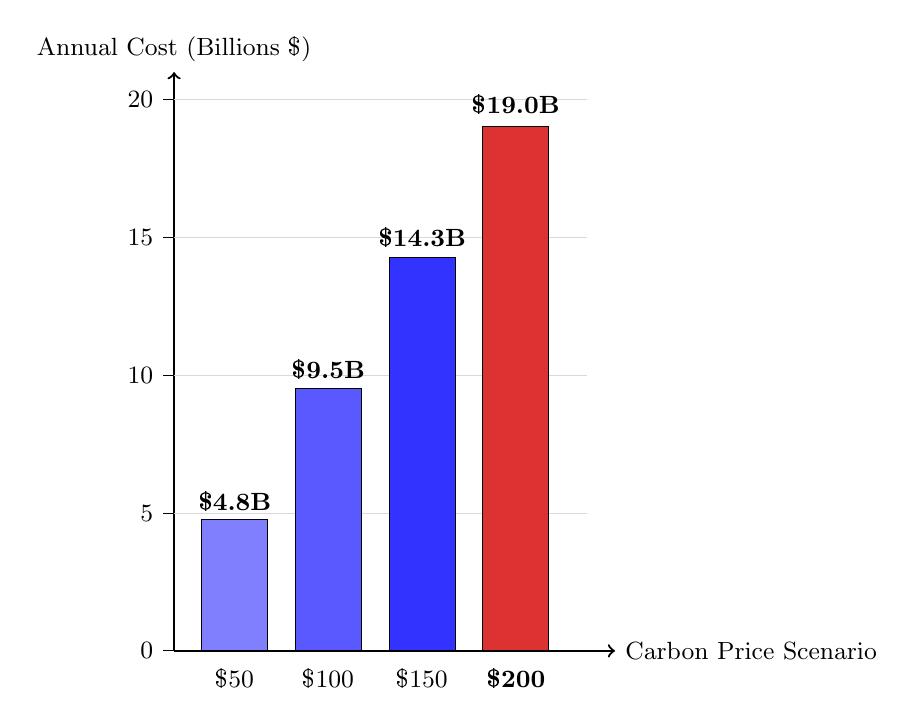
\begin{tikzpicture}[scale=0.7]
% Scale: 1 unit = 2 billion dollars, max height = 10 (for $20B)
% Values: $4.76B = 2.38, $9.52B = 4.76, $14.28B = 7.14, $19.04B = 9.52

% Y-axis
\draw[thick,->] (0,0) -- (0,10.5) node[above] {\small Annual Cost (Billions \$)};
% X-axis
\draw[thick,->] (0,0) -- (8,0) node[right] {\small Carbon Price Scenario};

% Y-axis labels
\foreach \y/\label in {0/0, 2.5/5, 5/10, 7.5/15, 10/20}
    \draw (0,\y) -- (-0.2,\y) node[left] {\small \label};

% Grid lines
\foreach \y in {2.5,5,7.5,10}
    \draw[gray!30,thin] (0,\y) -- (7.5,\y);

% Bars (width 1.2, spacing 0.3 between bars)
\draw[fill=blue!50] (0.5,0) rectangle (1.7,2.38);
\node[text=black, font=\bfseries\small] at (1.1,2.7) {\$4.8B};
\draw[fill=blue!65] (2.2,0) rectangle (3.4,4.76);
\node[text=black, font=\bfseries\small] at (2.8,5.1) {\$9.5B};
\draw[fill=blue!80] (3.9,0) rectangle (5.1,7.14);
\node[text=black, font=\bfseries\small] at (4.5,7.5) {\$14.3B};
\draw[fill=criticalred] (5.6,0) rectangle (6.8,9.52);
\node[text=black, font=\bfseries\small] at (6.2,9.9) {\$19.0B};

% X-axis labels
\node at (1.1,-0.5) {\small \$50};
\node at (2.8,-0.5) {\small \$100};
\node at (4.5,-0.5) {\small \$150};
\node at (6.2,-0.5) {\small \textbf{\$200}};
\end{tikzpicture}
\end{columns}
\end{frame}

% SLIDE 5: Risk Distribution
\begin{frame}{Key Finding \#2: Risk Distribution}
\begin{columns}[T]
\column{0.45\textwidth}
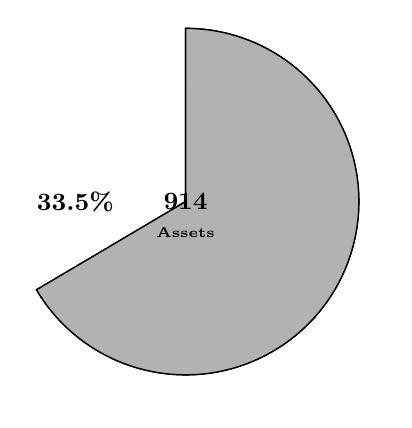
\begin{tikzpicture}[scale=1.0]
% Pie chart with accurate percentages and better colors
% Critical: 21/914 = 2.3% = 8.28 degrees (start at 90)
% High: 238/914 = 26.0% = 93.6 degrees
% Moderate: 342/914 = 37.4% = 134.64 degrees  
% Low: 7/914 = 0.8% = 2.88 degrees
% Closed: 306/914 = 33.5% = 120.6 degrees
\def\radius{2.2}
\coordinate (center) at (0,0);

% Start at 90 degrees (top), go clockwise
% Critical: 2.3% = 8.28° (90 to 81.72) - Red
\fill[fill=criticalred, draw=black, line width=0.5pt] (center) -- (90:\radius) arc (90:81.72:\radius) -- cycle;
\node[text=white, font=\bfseries\tiny] at (85.86:1.5) {2.3\%};

% High: 26.0% = 93.6° (81.72 to -11.88) - Yellow/Orange
\fill[fill=highyellow, draw=black, line width=0.5pt] (center) -- (81.72:\radius) arc (81.72:-11.88:\radius) -- cycle;
\node[text=black, font=\bfseries\small] at (34.92:1.6) {26.0\%};

% Moderate: 37.4% = 134.64° (-11.88 to -146.52) - Blue
\fill[fill=moderateblue, draw=black, line width=0.5pt] (center) -- (-11.88:\radius) arc (-11.88:-146.52:\radius) -- cycle;
\node[text=white, font=\bfseries\small] at (-79.2:1.5) {37.4\%};

% Low: 0.8% = 2.88° (-146.52 to -149.4) - Green
\fill[fill=lowgreen, draw=black, line width=0.5pt] (center) -- (-146.52:\radius) arc (-146.52:-149.4:\radius) -- cycle;
\node[text=white, font=\bfseries\tiny] at (-147.96:1.2) {0.8\%};

% Closed: 33.5% = 120.6° (-149.4 to 90, wrapping around) - Gray
\fill[fill=gray!60, draw=black, line width=0.5pt] (center) -- (-149.4:\radius) arc (-149.4:90:\radius) -- cycle;
\node[text=black, font=\bfseries\small] at (180:1.4) {33.5\%};

% Legend/center label
\node[text=black, font=\bfseries\small] at (center) {914};
\node[text=black, font=\bfseries\tiny] at (0,-0.4) {Assets};
\end{tikzpicture}

\vspace{0.3cm}

\centering
\small{\textbf{Risk at \$100/tCO\textsubscript{2}}}

\column{0.55\textwidth}
\begin{table}
\begin{tabular}{lrr}
\toprule
\textbf{Risk Level} & \textbf{Assets} & \textbf{\%} \\
\midrule
\textcolor{criticalred}{\textbf{Critical}} & 21 & 2.3\% \\
\textcolor{highyellow}{\textbf{High}} & 238 & 26.0\% \\
\textcolor{moderateblue}{\textbf{Moderate}} & 342 & 37.4\% \\
\textcolor{lowgreen}{\textbf{Low}} & 7 & 0.8\% \\
\midrule
\textit{Already Closed} & \textit{306} & \textit{33.5\%} \\
\midrule
\textbf{Total} & \textbf{914} & \textbf{100\%} \\
\bottomrule
\end{tabular}
\end{table}

\begin{alertblock}{Key Insight}
\textbf{259 assets} (28.3\%) require immediate strategic intervention\\
(Critical + High risk categories)
\end{alertblock}

\vspace{0.3cm}

\textbf{Most Vulnerable:}
\begin{itemize}
    \item El Salvador Mine (Chile): 39.5\% carbon/revenue
    \item Sepon Mine (Laos): 36.4\% carbon/revenue
\end{itemize}
\end{columns}
\end{frame}

% SLIDE 6: Screenshot 1 - Dashboard Overview
\begin{frame}{Interactive Dashboard: Overview}
\begin{center}
\includegraphics[width=0.95\textwidth]{../Screenshot 2026-01-03 at 21.57.38.png}
\end{center}

\vspace{0.3cm}

\begin{columns}[T]
\column{0.5\textwidth}
\textbf{Features:}
\begin{itemize}
    \item Real-time KPI cards
    \item Risk distribution visualization
    \item Scenario comparison
    \item Interactive asset explorer
\end{itemize}

\column{0.5\textwidth}
\textbf{Key Metrics Displayed:}
\begin{itemize}
    \item Total assets analyzed
    \item Carbon exposure by scenario
    \item Assets at risk percentage
    \item Critical assets count
\end{itemize}
\end{columns}
\end{frame}

% SLIDE 7: Screenshot 2 - Asset Analysis
\begin{frame}{Interactive Dashboard: Asset Analysis}
\begin{center}
\includegraphics[width=0.95\textwidth]{../Screenshot 2026-01-03 at 21.57.59.png}
\end{center}

\vspace{0.3cm}

\end{frame}

% SLIDE 8: Screenshot 3 - Geographic Mapping
\begin{frame}{Interactive Dashboard: Geographic Risk Mapping}
\begin{center}
\includegraphics[width=0.95\textwidth]{../Screenshot 2026-01-03 at 21.58.22.png}
\end{center}

\vspace{0.3cm}

\begin{columns}[T]
\column{0.5\textwidth}
\textbf{Geographic Insights:}
\begin{itemize}
    \item Global asset locations
    \item Risk overlays by region
    \item Interactive tooltips
    \item Concentration analysis
\end{itemize}

\column{0.5\textwidth}
\textbf{Top Countries:}
\begin{itemize}
    \item Chile: \$2.15B exposure
    \item DRC: \$1.52B exposure
    \item Peru: \$1.29B exposure
    \item Top 3 = 45.7\% of total
\end{itemize}
\end{columns}
\end{frame}

% SLIDE 9: Screenshot 4 - Scenario Analysis
\begin{frame}{Interactive Dashboard: Scenario Analysis}
\begin{center}
\includegraphics[width=0.95\textwidth]{../Screenshot 2026-01-03 at 21.58.36.png}
\end{center}

\vspace{0.3cm}

\begin{columns}[T]
\column{0.5\textwidth}
\textbf{Scenario Modeling:}
\begin{itemize}
    \item 4 carbon pricing scenarios
    \item Trajectory projections (2025-2040)
    \item Monte Carlo simulations
    \item Value-at-Risk metrics
\end{itemize}

\column{0.5\textwidth}
\textbf{Scenarios:}
\begin{itemize}
    \item Orderly Transition
    \item Disorderly Transition
    \item Hothouse World
    \item Uncertainty bands
\end{itemize}
\end{columns}
\end{frame}

% SLIDE 10: Screenshot 5 - Risk Categories
\begin{frame}{Interactive Dashboard: Risk Categories}
\begin{center}
\includegraphics[width=0.95\textwidth]{../Screenshot 2026-01-03 at 21.58.57.png}
\end{center}

\vspace{0.3cm}

\begin{columns}[T]
\column{0.5\textwidth}
\textbf{Risk Panels:}
\begin{itemize}
    \item Critical risk assets
    \item Divestment candidates
    \item Low-risk opportunities
    \item Action recommendations
\end{itemize}

\column{0.5\textwidth}
\textbf{Portfolio Actions:}
\begin{itemize}
    \item Immediate intervention needed
    \item Strategic divestments
    \item Investment opportunities
    \item Decarbonization priorities
\end{itemize}
\end{columns}
\end{frame}

% SLIDE 11: Key Finding - Emissions Trends
\begin{frame}{Key Finding \#3: Emissions Trending Upward}
\begin{columns}[T]
\column{0.5\textwidth}
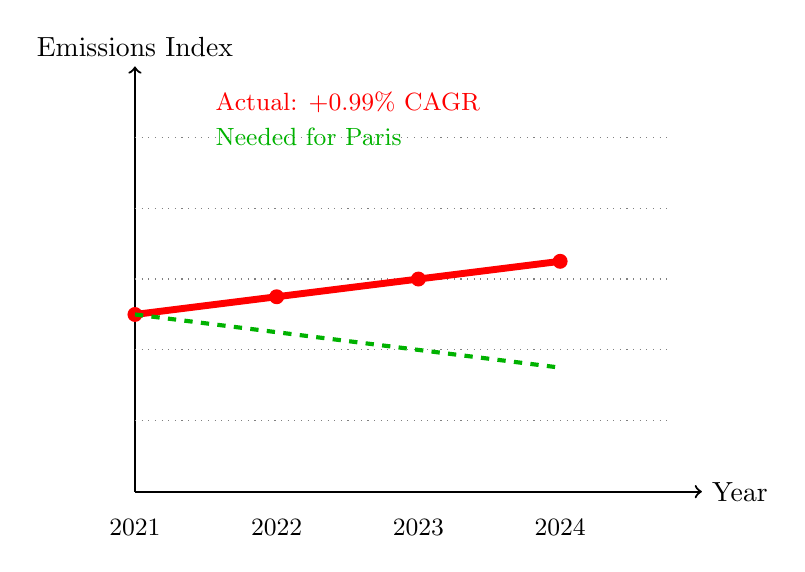
\begin{tikzpicture}[scale=0.9]
\draw[thick,->] (0,0) -- (8,0) node[right] {Year};
\draw[thick,->] (0,0) -- (0,6) node[above] {Emissions Index};

% Grid
\foreach \y in {1,2,3,4,5}
    \draw[gray,dotted] (0,\y) -- (7.5,\y);

% Main trend line (red, going up)
\draw[thick,red,line width=2.5pt] plot coordinates {
    (0,2.5) (2,2.75) (4,3.0) (6,3.25)
};
\fill[red] (0,2.5) circle (3pt);
\fill[red] (2,2.75) circle (3pt);
\fill[red] (4,3.0) circle (3pt);
\fill[red] (6,3.25) circle (3pt);

% Reference line (what should be happening)
\draw[thick,green!70!black,dashed,line width=1.5pt] plot coordinates {
    (0,2.5) (2,2.25) (4,2.0) (6,1.75)
};

% Labels
\node at (0,-0.5) {\small 2021};
\node at (2,-0.5) {\small 2022};
\node at (4,-0.5) {\small 2023};
\node at (6,-0.5) {\small 2024};

% Legend
\node[right, red] at (1,5.5) {\small Actual: +0.99\% CAGR};
\node[right, green!70!black] at (1,5) {\small Needed for Paris};
\end{tikzpicture}

\column{0.5\textwidth}
\textbf{Trajectory Analysis:}

\vspace{0.3cm}

\begin{table}
\begin{tabular}{lr}
\toprule
\textbf{Trend} & \textbf{Assets} \\
\midrule
\rowcolor{criticalred!20}
Deteriorating ($>$10\% ↑) & 202 \\
Improving ($>$10\% ↓) & 119 \\
Stable ($\pm$10\%) & 208 \\
\bottomrule
\end{tabular}
\end{table}

\vspace{0.5cm}

\begin{alertblock}{Critical Problem}
\textbf{202 assets} have worsening emissions\\
Industry moving \textit{away} from decarbonization
\end{alertblock}

\vspace{0.3cm}


\end{columns}
\end{frame}

% SLIDE 12: Company Exposure
\begin{frame}{Key Finding \#4: Company-Level Exposure}
\begin{columns}[T]
\column{0.55\textwidth}
\textbf{Top 10 Companies by Carbon Cost}

\vspace{0.3cm}

\begin{table}
\small
\begin{tabular}{llr}
\toprule
\textbf{Rank} & \textbf{Company} & \textbf{\$M @ \$100} \\
\midrule
1 & \textbf{Freeport-McMoRan} & \textbf{1,245} \\
2 & \textbf{Codelco} & \textbf{1,123} \\
3 & \textbf{BHP} & \textbf{987} \\
4 & Rio Tinto & 876 \\
5 & Glencore & 845 \\
6 & Southern Copper & 678 \\
7 & Anglo American & 534 \\
8 & First Quantum & 498 \\
9 & Antofagasta & 445 \\
10 & Teck Resources & 389 \\
\midrule
& \textbf{Top 10 Total} & \textbf{7,620} \\
\bottomrule
\end{tabular}
\end{table}

\column{0.45\textwidth}
\begin{alertblock}{Concentration}
Top 10 companies = \textbf{80\%} of industry exposure
\end{alertblock}

\vspace{0.5cm}

\textbf{Investor Implications:}
\begin{itemize}
    \item Major portfolio companies at risk
    \item ESG ratings will reflect exposure
    \item Shareholder pressure mounting
    \item Divestment risk for worst performers
\end{itemize}

\vspace{0.5cm}

\textbf{Company Response Needed:}
\begin{itemize}
    \item Asset-level decarbonization plans
    \item Renewable energy investment
    \item Strategic divestments
\end{itemize}
\end{columns}
\end{frame}

% SLIDE 13: Machine Learning
\begin{frame}{Key Finding \#5: Predictive Risk Modeling}
\begin{columns}[T]
\column{0.5\textwidth}
\textbf{Random Forest Model}

\vspace{0.3cm}

\begin{table}
\begin{tabular}{lr}
\toprule
\textbf{Metric} & \textbf{Score} \\
\midrule
Accuracy & 84.2\% \\
Precision & 79.3\% \\
Recall & 72.7\% \\
ROC-AUC & 0.87 \\
\bottomrule
\end{tabular}
\end{table}

\vspace{0.5cm}

\textbf{Feature Importance:}
\begin{itemize}
    \item Carbon Intensity: 31\%
    \item Capacity Factor: 24\%
    \item Production Volume: 18\%
    \item Temporal Trend: 12\%
    \item Other factors: 15\%
\end{itemize}

\column{0.5\textwidth}
\textbf{What This Enables:}

\vspace{0.5cm}

\begin{block}{Proactive Risk Management}
Predict which assets will become stranded \textit{before} they fail
\end{block}

\vspace{0.5cm}

\textbf{Use Cases:}
\begin{enumerate}
    \item \textbf{Portfolio optimization}\\
    Divest high-risk assets early

    \item \textbf{Targeted interventions}\\
    Focus capex on saveable assets

    \item \textbf{Valuation adjustments}\\
    Price carbon risk into M\&A

    \item \textbf{Insurance pricing}\\
    Risk-based carbon insurance
\end{enumerate}
\end{columns}
\end{frame}

% SLIDE 14: Recommendations
\begin{frame}{Recommendations}
\begin{columns}[T]
\column{0.5\textwidth}
\textbf{Mining Companies}

\vspace{0.3cm}

\begin{enumerate}
    \item \textbf{Immediate audit}\\
    Assess 259 critical/high-risk assets

    \item \textbf{Divest underwater assets}\\
    El Salvador, Sepon already unviable

    \item \textbf{Decarbonization capex}\\
    Prioritize open pit electrification

    \item \textbf{Renewable PPAs}\\
    Lock in green power for processing

    \item \textbf{Enhanced disclosure}\\
    Asset-level carbon reporting
\end{enumerate}

\column{0.5\textwidth}
\textbf{Investors \& Lenders}

\vspace{0.3cm}

\begin{enumerate}
    \item \textbf{Portfolio stress testing}\\
    Model \$150-200 carbon scenarios

    \item \textbf{Engagement campaigns}\\
    Demand decarbonization plans

    \item \textbf{Credit risk repricing}\\
    Adjust spreads for carbon exposure

    \item \textbf{Thematic opportunities}\\
    Low-carbon copper as alpha source

    \item \textbf{Voting actions}\\
    Support climate resolutions
\end{enumerate}

\vspace{0.5cm}

\textbf{Policymakers}
\begin{itemize}
    \item Predictable carbon price escalation
    \item Just transition support for workers
    \item R\&D funding for mine electrification
\end{itemize}
\end{columns}
\end{frame}

% SLIDE 15: Conclusion
\begin{frame}{Conclusion}
\begin{center}
\Large \textbf{The copper mining industry faces a \$19B annual carbon crisis}

\vspace{1cm}

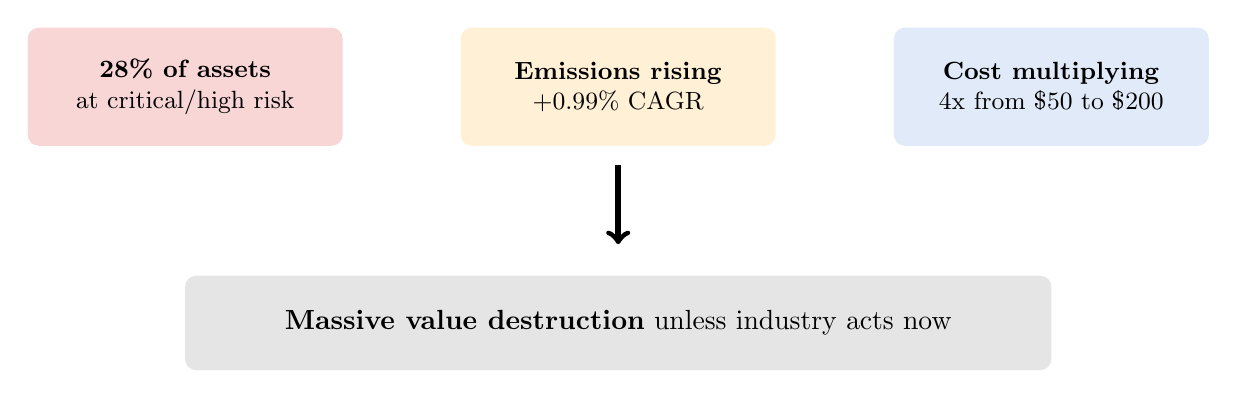
\begin{tikzpicture}
% Three boxes showing the problem
\node[fill=criticalred!20, rounded corners, minimum width=4cm, minimum height=1.5cm, align=center, font=\small] at (0,0)
{\textbf{28\% of assets}\\at critical/high risk};

\node[fill=highyellow!20, rounded corners, minimum width=4cm, minimum height=1.5cm, align=center, font=\small] at (5.5,0)
{\textbf{Emissions rising}\\+0.99\% CAGR};

\node[fill=moderateblue!20, rounded corners, minimum width=4cm, minimum height=1.5cm, align=center, font=\small] at (11,0)
{\textbf{Cost multiplying}\\4x from \$50 to \$200};

% Arrow pointing down
\draw[->,thick,line width=2pt] (5.5,-1) -- (5.5,-2);

% Bottom consequence box
\node[fill=gray!20, rounded corners, minimum width=11cm, minimum height=1.2cm, align=center, font=\normalsize] at (5.5,-3)
{\textbf{Massive value destruction} unless industry acts now};
\end{tikzpicture}

\vspace{1cm}

\normalsize
\textbf{This is not a distant threat.} Carbon prices are already rising.\\
Assets are already becoming uneconomic.

\vspace{0.5cm}

\textbf{Our analysis provides:}
\begin{itemize}
    \item Comprehensive risk assessment across 914 assets
    \item Interactive tools for decision-making
    \item Predictive models for proactive management
    \item Actionable recommendations for all stakeholders
\end{itemize}
\end{center}
\end{frame}

% SLIDE 16: Thank You
\begin{frame}
\begin{center}
\Huge Thank You

\vspace{1.5cm}

\vspace{1cm}

\normalsize
\textbf{Alexis Vannson, Kerrian Le Bars and Othmane Menkor}\\
Research Emerging Topics\\
January 2026

\vspace{1cm}

\begin{tabular}{rl}
\textbf{Data:} & Climate TRACE v5.2.0 \\
\textbf{Assets Analyzed:} & 914 global copper mines \\
\end{tabular}
\end{center}
\end{frame}

\end{document}

